% Grouped bar chart — paper_simple_boosted_20260627 benchmark results
%
% Level | Optimal | Min solutionLength | MOMoT block count
%     1 |       2 |                  2 |                 2
%     2 |       5 |                  8 |                 8
%     3 |       2 |                  2 |                 2
%     4 |       5 |                 11 |                 8
%     5 |       5 |                  8 |                 8
%     6 |       4 |                 10 |                 9
%     7 |       4 |                  8 |                 6
%     8 |       5 |                 12 |                11
%     9 |       4 |                  8 |                 5
%    10 |       7 |                 38 |                10

\documentclass[tikz,border=5pt]{standalone}

\usepackage{pgfplots}
\pgfplotsset{compat=1.18}

\definecolor{optimalblue}{RGB}{31,119,180}
\definecolor{transformorange}{RGB}{255,127,14}
\definecolor{blockgreen}{RGB}{44,160,44}

\begin{document}

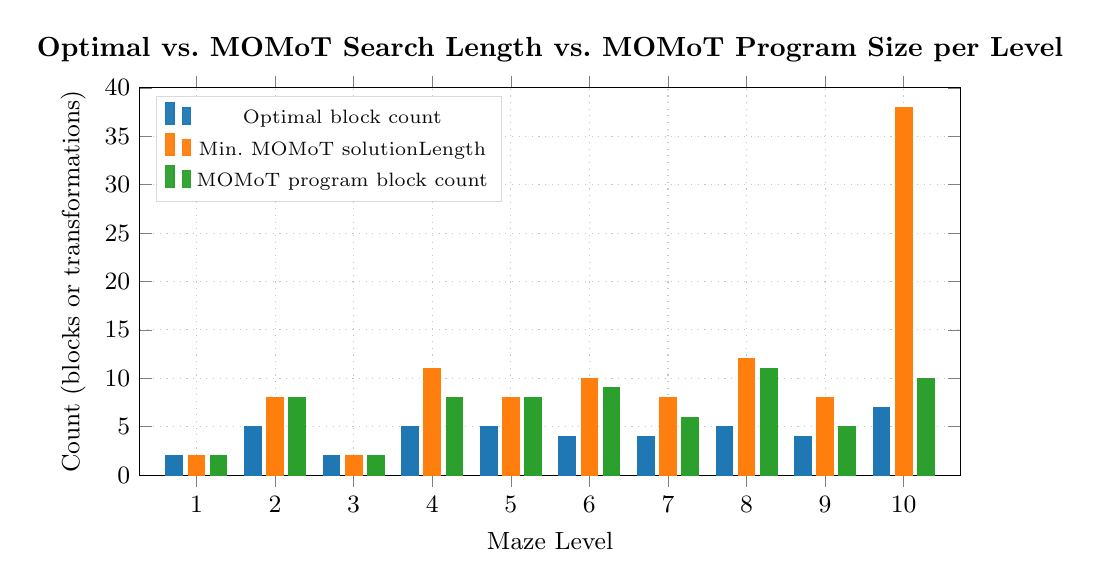
\begin{tikzpicture}
\begin{axis}[
    width=12cm,
    height=6.5cm,
    ybar,
    bar width=6pt,
    enlarge x limits=0.08,
    ymin=0,
    ymax=40,
    ytick={0,5,10,15,20,25,30,35,40},
    grid=major,
    major grid style={dotted, draw=gray!45},
    minor y tick num=0,
    xlabel={Maze Level},
    ylabel={Count (blocks or transformations)},
    title={Optimal vs.\ MOMoT Search Length vs.\ MOMoT Program Size per Level},
    title style={font=\bfseries},
    symbolic x coords={1,2,3,4,5,6,7,8,9,10},
    xtick=data,
    legend style={
        at={(0.02,0.98)},
        anchor=north west,
        fill=white,
        fill opacity=0.95,
        draw=gray!30,
        font=\scriptsize,
    },
    tick label style={font=\small},
    label style={font=\small},
]

\addplot[
    fill=optimalblue,
    draw=optimalblue,
    bar shift=-8pt,
] coordinates {
    (1,2) (2,5) (3,2) (4,5) (5,5) (6,4) (7,4) (8,5) (9,4) (10,7)
};

\addplot[
    fill=transformorange,
    draw=transformorange,
] coordinates {
    (1,2) (2,8) (3,2) (4,11) (5,8) (6,10) (7,8) (8,12) (9,8) (10,38)
};

\addplot[
    fill=blockgreen,
    draw=blockgreen,
    bar shift=8pt,
] coordinates {
    (1,2) (2,8) (3,2) (4,8) (5,8) (6,9) (7,6) (8,11) (9,5) (10,10)
};

\legend{Optimal block count, Min.\ MOMoT solutionLength, MOMoT program block count}

\end{axis}
\end{tikzpicture}

\end{document}
